%----------------------------------------------------------------------------------------
%	Compilar en PC con LuaLatex.
%	TeXstudio: Opciones>Configurar TeXstudio
%----------------------------------------------------------------------------------------
\documentclass[
10pt,			% Main document font size
letterpaper,	% Paper type, use 'a4paper' for a4 Letter paper
oneside,		% One page layout (no page indentation)
%twoside,		% Two page layout (page indentation for binding and different headers)
headinclude, footinclude, % Extra spacing for the header and footer
BCOR5mm, 		% Binding correction
]{scrartcl}

\usepackage[
nochapters, % Turn off chapters since this is an article        
beramono, % Use the Bera Mono font for monospaced text (\texttt)
eulermath,% Use the Euler font for mathematics
pdfspacing, % Makes use of pdftex’ letter spacing capabilities via the microtype package
dottedtoc % Dotted lines leading to the page numbers in the table of contents
]{classicthesis} % The layout is based on the Classic Thesis style

%----------------------------------------------------------------------------------------
%	Codification text & symbols
%----------------------------------------------------------------------------------------
\usepackage[utf8]{inputenc}		% Required for including letters with accents
\usepackage[T1]{fontenc}		% Use 8-bit encoding that has 256 glyphs
\usepackage[spanish]{babel}		% Español %\usepackage[spanish]{layout}
\usepackage{arsclassica}		% Modifies the Classic Thesis package
%----------------------------------------------------------------------------------------
%	Varios Required Packages
%----------------------------------------------------------------------------------------
\usepackage{comment}			% Agregar comentarios
\usepackage{lipsum}				% Inserts dummy text
\usepackage{enumitem}			% Customize lists
\setlist[description]{style=nextline}
\usepackage{blindtext}			% Inserts random paragraph \blindtext
\usepackage{etoolbox}			% Conditional macros
\setlist{nolistsep}				% Reduce spacing between bullet points and numbered lists
%----------------------------------------------------------------------------------------
%	Colours Packages
%----------------------------------------------------------------------------------------
\usepackage{xcolor}										% Specifying colors by name
%\usepackage[table,x11names,dvipsnames,table]{xcolor}	% \usepackage{xcolor}%Specifying colors by name
%\usepackage[colorlinks=true, urlcolor=ocre]{hyperref}	% Forinserting hyperlinks (colours)
\usepackage{tcolorbox}									% Coloured boxes, for LATEX examples and theorems, etc
\usepackage{color}										% Color packages foreground and back­ground color man­age­ment
%----------------------------------------------------------------------------------------
%	Text and fonts
%----------------------------------------------------------------------------------------
\usepackage{textcomp}					% Text Companion fonts, which provide many text symbols
\usepackage{titlesec}					% Allows customization of titles
\usepackage{verbatim}					% Verbatim
\usepackage{microtype}					% Slightly tweak font spacing for aesthetics
\usepackage{avant}						% Use the Avantgarde font for headings
\RequirePackage{fix-cm}					% permit Computer Modern fonts at arbitrary sizes.
\usepackage{calc}						% For simpler calculation - used for spacing the index letter headings correctly
\usepackage[labelsep=endash]{caption}	% Type of separation Caption\usepackage{caption}
\usepackage{caption}
\usepackage{textcomp}					%
\usepackage{setspace}					% 
\usepackage{listings}					% Coding
\usepackage[framed,numbered,autolinebreaks,useliterate]{./structure/mcode}
%\usepackage{./structure/mcode}			%
\usepackage{times}						% Use the Times font for headings
\usepackage{lmodern}					%
\usepackage{marvosym}					%
\usepackage{gensymb}					%
\usepackage{mathpazo}					% \textonehalf, \textonequarter, \textthreequarters.
\usepackage{textcomp}					%
%\usepackage{kpfonts}					% 
%----------------------------------------------------------------------------------------
%	Tables
%----------------------------------------------------------------------------------------
\usepackage{multicol}
\usepackage{bigstrut}
\usepackage{multirow}       % Allow table cells to span multiple rows
\usepackage{threeparttable} % tables with footnotes, capions all the same width
\usepackage{dcolumn}        % decimal-aligned tabular math columns
\usepackage{booktabs}       % Publication-quality tables -nicer horizontal rules in tables
\usepackage{ltxtable}       % long tabularx
\usepackage{tabularx}
\usepackage{tabulary}
\usepackage{colortbl}		% colured ‘panels’ behind specified columns in a table.
\usepackage{makecell}		% Celdas con diagonales
\usepackage{longtable}		% Длинные таблицы
%----------------------------------------------------------------------------------------
%	Image packages
%----------------------------------------------------------------------------------------
\usepackage[margin=1in]{geometry}
\usepackage{graphicx}			% Required for including pictures
\usepackage{graphics}			% 
\usepackage{subfig}				% Required for creating figures with multiple parts (subfigures)
\usepackage{tikz}				% Required for drawing custom shapes
\usetikzlibrary{matrix}			%
\usetikzlibrary{circuits}		%
\usetikzlibrary{arrows,shapes}	%
\usetikzlibrary{chains}			%
%\usetikzlibrary{dsp}			%
\usetikzlibrary{backgrounds}	
\usepackage{float}
\usepackage{subfloat}
\usepackage{placeins}
\usepackage[siunitx]{circuitikz}
\usepackage{schemabloc}
\usepackage{epstopdf}
\usepackage{eso-pic}			% Required for specifying an image background in the title page
%----------------------------------------------------------------------------------------
%	Math packages
%----------------------------------------------------------------------------------------
\usepackage{amsmath,amssymb,amsthm}		% For including math equations, theorems, symbols, etc
\usepackage{amsfonts}
\usepackage{dsfont}
\usepackage{array}
\usepackage{eqnarray}
\usepackage{cases}						% function defined piecewise
\usepackage{mathtools}
\usepackage{mathptmx}					% AdobeTimesRoman as the default text font with mathsymb from Sym­bol/Chancery/Com­puterModernfonts
\usepackage{bm}							% bold math symbols $\alpha \not= \bm{\alpha}$
\usepackage{nicefrac}					%
\usepackage{xfrac}
\usepackage{mathrsfs}
%----------------------------------------------------------------------------------------
%	Bibliography, References and Index
%----------------------------------------------------------------------------------------
%\usepackage[dcucite]{harvard}		%bibliography style, dcu gives commas before year, semicolon between references, and "and" between authors
%\usepackage{html}					% To get harvard to work, insert immediately before \usepackage{harvard}
%\usepackage{url}					% To get harvard to work, insert immediately before \title{...}
%\usepackage{cite}
%\usepackage{cleveref}				% Dice donde esta lo referenciado
%\hyphenation{Fortran hy-phen-ation} % Specify custom hyphenation points in words with dashes where you would like hyphenation to occur
\usepackage{varioref}				% More descriptive referencing
%\parindent=0pt
%\usepackage{makeidx} % Required to make an index
%\makeindex % Tells LaTeX to create the files required for indexing 
%\usepackage[colorlinks=true, urlcolor=ocre]{hyperref} % Forinserting hyperlinks (colours)
%\usepackage{hyperref}
%%----------------------------------------------------------------------------------------
%	MAIN TABLE OF CONTENTS
%----------------------------------------------------------------------------------------
\usepackage{titletoc} % Required for manipulating the table of contents
\contentsmargin{0cm} % Removes the default margin
% Part text styling
\titlecontents{part}[0cm]
{\addvspace{20pt}\centering\large\bfseries}
{}
{}
{}
% Chapter text styling
\titlecontents{chapter}[1.25cm] % Indentation
{\addvspace{15pt}\large\sffamily\bfseries} % Spacing and font options for chapters
{\color{ocre!60}\contentslabel[\Large\thecontentslabel]{1.25cm}\color{ocre}} % Chapter number
{}
{\color{ocre!60}\normalsize\sffamily\bfseries\;\titlerule*[.5pc]{.}\;\thecontentspage} % Page number
%{\color{ocre!60}\normalsize\;\titlerule*[.5pc]{.}\;\thecontentspage} % Page number

% Section text styling
\titlecontents{section}[1.25cm] % Indentation
{\addvspace{5pt}\sffamily\bfseries} % Spacing and font options for sections
{\contentslabel[\thecontentslabel]{1.25cm}} % Section number
{}
{\sffamily\hfill\color{black}\thecontentspage} % Page number
%{\hfill\color{black}\thecontentspage} % Page number
[]
% Subsection text styling
\titlecontents{subsection}[1.25cm] % Indentation
{\addvspace{1pt}\sffamily\small} % Spacing and font options for subsections
{\contentslabel[\thecontentslabel]{1.25cm}} % Subsection number
{}
{\sffamily\;\titlerule*[.5pc]{.}\;\thecontentspage} % Page number
%{\ \titlerule*[.5pc]{.}\;\thecontentspage} % Page number
[] 
% List of figures
\titlecontents{figure}[0em]
{\addvspace{-5pt}\sffamily}
{\thecontentslabel\hspace*{1em}}
{}
{\ \titlerule*[.5pc]{.}\;\thecontentspage}
[]
% List of taibles
\titlecontents{table}[0em]
{\addvspace{-5pt}\sffamily}
{\thecontentslabel\hspace*{1em}}
{}
{\ \titlerule*[.5pc]{.}\;\thecontentspage}
[]
%----------------------------------------------------------------------------------------
%	MINI TABLE OF CONTENTS IN CHAPTER HEADS
%----------------------------------------------------------------------------------------
 % Chapter text styling
\titlecontents{lchapter}[0em] % Indenting
{\addvspace{15pt}\large\sffamily\bfseries} % Spacing and font options for chapters
{\color{ocre}\contentslabel[\Large\thecontentslabel]{1.25cm}\color{ocre}} % Chapter number
{}  
{\color{ocre}\normalsize\sffamily\bfseries\;\titlerule*[.5pc]{.}\;\thecontentspage} % Page number
% Section text styling
\titlecontents{lsection}[0em] % Indendating
%{\footnotesize\sffamily} % Font settings 
{\sffamily\small} % Spacing and font options for sections
{\contentslabel[\thecontentslabel]{1.25cm}} % Section number
%{}
{}
{}
% Subsection text styling
\titlecontents{lsubsection}[.5em] % Indentation
{\normalfont\footnotesize\sffamily} % Font settings
{}
{}
{}
%----------------------------------------------------------------------------------------
%	PAGE HEADERS
%----------------------------------------------------------------------------------------
\usepackage{fancyhdr} % Required for header and footer configuration
\pagestyle{fancy}
\renewcommand{\chaptermark}[1]{\markboth{\sffamily\normalsize\bfseries\chaptername\ \thechapter.\ #1}{}} % Chapter text font settings
\renewcommand{\sectionmark}[1]{\markright{\sffamily\normalsize\thesection\hspace{5pt}#1}{}} % Section text font settings
\fancyhf{} \fancyhead[LE,RO]{\sffamily\normalsize\thepage} % Font setting for the page number in the header
\fancyhead[LO]{\rightmark} % Print the nearest section name on the left side of odd pages
\fancyhead[RE]{\leftmark} % Print the current chapter name on the right side of even pages
\renewcommand{\headrulewidth}{0.5pt} % Width of the rule under the header
\addtolength{\headheight}{2.5pt} % Increase the spacing around the header slightly
\renewcommand{\footrulewidth}{0pt} % Removes the rule in the footer
\fancypagestyle{plain}{\fancyhead{}\renewcommand{\headrulewidth}{0pt}} % Style for when a plain pagestyle is specified
% Removes the header from odd empty pages at the end of chapters
\makeatletter
\renewcommand{\cleardoublepage}{
\clearpage\ifodd\c@page\else
\hbox{}
\vspace*{\fill}
\thispagestyle{empty}
\newpage
\fi}
%----------------------------------------------------------------------------------------
%	THEOREM STYLES
%----------------------------------------------------------------------------------------
\newcommand{\intoo}[2]{\mathopen{]}#1\,;#2\mathclose{[}}
\newcommand{\ud}{\mathop{\mathrm{{}d}}\mathopen{}}
\newcommand{\intff}[2]{\mathopen{[}#1\,;#2\mathclose{]}}
\newtheorem{notation}{Notación}[chapter]



%%%%%%%%%%%%%%%%%%%%%%%%%%%%%%%%%%%%%%%%%%%%%%%%%%%%%%%%%%%%%%%%%%%%%%%%%%%
%%%%%%%%%%%%%%%%%%%% dedicated to boxed/framed environements %%%%%%%%%%%%%%
%%%%%%%%%%%%%%%%%%%%%%%%%%%%%%%%%%%%%%%%%%%%%%%%%%%%%%%%%%%%%%%%%%%%%%%%%%%
\newtheoremstyle{ocrenumbox}% % Theorem style name
{0pt}% Space above
{0pt}% Space below
{\normalfont}% % Body font
{}% Indent amount
{\small\bf\sffamily\color{ocre}}% % Theorem head font
{\;}% Punctuation after theorem head
{0.25em}% Space after theorem head
{\small\sffamily\color{ocre}\thmname{#1}\nobreakspace\thmnumber{\@ifnotempty{#1}{}\@upn{#2}}% Theorem text (e.g. Theorem 2.1)
\thmnote{\nobreakspace\the\thm@notefont\sffamily\bfseries\color{black}---\nobreakspace#3.}} % Optional theorem note
\renewcommand{\qedsymbol}{$\blacksquare$}% Optional qed square
\newtheoremstyle{blacknumex}% Theorem style name
{5pt}% Space above
{5pt}% Space below
{\normalfont}% Body font
{} % Indent amount
{\small\bf\sffamily}% Theorem head font
{\;}% Punctuation after theorem head
{0.25em}% Space after theorem head
{\small\sffamily{\tiny\ensuremath{\blacksquare}}\nobreakspace\thmname{#1}\nobreakspace\thmnumber{\@ifnotempty{#1}{}\@upn{#2}}% Theorem text (e.g. Theorem 2.1)
\thmnote{\nobreakspace\the\thm@notefont\sffamily\bfseries---\nobreakspace#3.}}% Optional theorem note
\newtheoremstyle{blacknumbox} % Theorem style name
{0pt}% Space above
{0pt}% Space below
{\normalfont}% Body font
{}% Indent amount
{\small\bf\sffamily}% Theorem head font
{\;}% Punctuation after theorem head
{0.25em}% Space after theorem head
{\small\sffamily\thmname{#1}\nobreakspace\thmnumber{\@ifnotempty{#1}{}\@upn{#2}}% Theorem text (e.g. Theorem 2.1)
\thmnote{\nobreakspace\the\thm@notefont\sffamily\bfseries---\nobreakspace#3.}}% Optional theorem note
%%%%%%%%%%%%%%%%%%%%%%%%%%%%%%%%%%%%%%%%%%%%%%%%%%%%%%%%%%%%%%%%%%%%%%%%%%%
%%%%%%%%%%%%% dedicated to non-boxed/non-framed environements %%%%%%%%%%%%%
%%%%%%%%%%%%%%%%%%%%%%%%%%%%%%%%%%%%%%%%%%%%%%%%%%%%%%%%%%%%%%%%%%%%%%%%%%%
\newtheoremstyle{ocrenum}% % Theorem style name
{5pt}% Space above
{5pt}% Space below
{\normalfont}% % Body font
{}% Indent amount
{\small\bf\sffamily\color{ocre}}% % Theorem head font
{\;}% Punctuation after theorem head
{0.25em}% Space after theorem head
{\small\sffamily\color{ocre}\thmname{#1}\nobreakspace\thmnumber{\@ifnotempty{#1}{}\@upn{#2}}% Theorem text (e.g. Theorem 2.1)
\thmnote{\nobreakspace\the\thm@notefont\sffamily\bfseries\color{black}---\nobreakspace#3.}} % Optional theorem note
\renewcommand{\qedsymbol}{$\blacksquare$}% Optional qed square
\makeatother
% Defines the theorem text style for each type of theorem to one of the three styles above
\newcounter{dummy} 
\numberwithin{dummy}{section}
\theoremstyle{ocrenumbox}
\newtheorem{theoremeT}[dummy]{Teorema}
\newtheorem{problem}{Problema}[chapter]
\newtheorem{exerciseT}{Ejercicio}[chapter]
\theoremstyle{blacknumex}
\newtheorem{exampleT}{Ejemplo}[chapter]
\theoremstyle{blacknumbox}
\newtheorem{vocabulary}{Vocabulario}[chapter]
\newtheorem{definitionT}{Definición}[section]
\newtheorem{corollaryT}[dummy]{Corollary}
\theoremstyle{ocrenum}
\newtheorem{proposition}[dummy]{Proposición}

%----------------------------------------------------------------------------------------
%	DEFINITION OF COLORED BOXES
%----------------------------------------------------------------------------------------
\RequirePackage[framemethod=default]{mdframed} % Required for creating the theorem, definition, exercise and corollary boxes

% Theorem box
\newmdenv[skipabove=7pt,
skipbelow=7pt,
backgroundcolor=black!5,
linecolor=ocre,
innerleftmargin=5pt,
innerrightmargin=5pt,
innertopmargin=5pt,
leftmargin=0cm,
rightmargin=0cm,
innerbottommargin=5pt]{tBox}

% Exercise box	  
\newmdenv[skipabove=7pt,
skipbelow=7pt,
rightline=false,
leftline=true,
topline=false,
bottomline=false,
backgroundcolor=ocre!10,
linecolor=ocre,
innerleftmargin=5pt,
innerrightmargin=5pt,
innertopmargin=5pt,
innerbottommargin=5pt,
leftmargin=0cm,
rightmargin=0cm,
linewidth=4pt]{eBox}	

% Definition box
\newmdenv[skipabove=7pt,
skipbelow=7pt,
rightline=false,
leftline=true,
topline=false,
bottomline=false,
linecolor=ocre,
innerleftmargin=5pt,
innerrightmargin=5pt,
innertopmargin=0pt,
leftmargin=0cm,
rightmargin=0cm,
linewidth=4pt,
innerbottommargin=0pt]{dBox}	

% Corollary box
\newmdenv[skipabove=7pt,
skipbelow=7pt,
rightline=false,
leftline=true,
topline=false,
bottomline=false,
linecolor=gray,
backgroundcolor=black!5,
innerleftmargin=5pt,
innerrightmargin=5pt,
innertopmargin=5pt,
leftmargin=0cm,
rightmargin=0cm,
linewidth=4pt,
innerbottommargin=5pt]{cBox}

% Creates an environment for each type of theorem and assigns it a theorem text style from the "Theorem Styles" section above and a colored box from above
\newenvironment{theorem}{\begin{tBox}\begin{theoremeT}}{\end{theoremeT}\end{tBox}}
\newenvironment{exercise}{\begin{eBox}\begin{exerciseT}}{\hfill{\color{ocre}\tiny\ensuremath{\blacksquare}}\end{exerciseT}\end{eBox}}				  
\newenvironment{definition}{\begin{dBox}\begin{definitionT}}{\end{definitionT}\end{dBox}}	
\newenvironment{example}{\begin{exampleT}}{\hfill{\tiny\ensuremath{\blacksquare}}\end{exampleT}}		
\newenvironment{corollary}{\begin{cBox}\begin{corollaryT}}{\end{corollaryT}\end{cBox}}	

%----------------------------------------------------------------------------------------
%	REMARK ENVIRONMENT
%----------------------------------------------------------------------------------------
\newenvironment{remark}{\par\vspace{10pt}\small % Vertical white space above the remark and smaller font size
\begin{list}{}{
\leftmargin=35pt % Indentation on the left
\rightmargin=25pt}\item\ignorespaces % Indentation on the right
\makebox[-2.5pt]{\begin{tikzpicture}[overlay]
\node[draw=ocre!60,line width=1pt,circle,fill=ocre!25,font=\sffamily\bfseries,inner sep=2pt,outer sep=0pt] at (-15pt,0pt){\textcolor{ocre}{N}};\end{tikzpicture}} % Orange R in a circle
\advance\baselineskip -1pt}{\end{list}\vskip5pt} % Tighter line spacing and white space after remark

%----------------------------------------------------------------------------------------
%	SECTION NUMBERING IN THE MARGIN
%----------------------------------------------------------------------------------------
\makeatletter
\renewcommand{\@seccntformat}[1]{\llap{\textcolor{ocre}{\csname the#1\endcsname}\hspace{1em}}}                    
\renewcommand{\section}{\@startsection{section}{1}{\z@}
	{-4ex \@plus -1ex \@minus -.4ex}
	{1ex \@plus.2ex }
	{\normalfont\large\sffamily\bfseries}}
\renewcommand{\subsection}{\@startsection {subsection}{2}{\z@}
	{-3ex \@plus -0.1ex \@minus -.4ex}
	{0.5ex \@plus.2ex }
	{\normalfont\sffamily\bfseries}}
\renewcommand{\subsubsection}{\@startsection {subsubsection}{3}{\z@}
	{-2ex \@plus -0.1ex \@minus -.2ex}
	{.2ex \@plus.2ex }
	{\normalfont\small\sffamily\bfseries}}                        
\renewcommand\paragraph{\@startsection{paragraph}{4}{\z@}
	{-2ex \@plus-.2ex \@minus .2ex}
	{.1ex}
	{\normalfont\small\sffamily\bfseries}}

%----------------------------------------------------------------------------------------
%	PART HEADINGS
%----------------------------------------------------------------------------------------
% numbered part in the table of contents
\newcommand{\@mypartnumtocformat}[2]{%
	\setlength\fboxsep{0pt}%
	\noindent\colorbox{ocre!20}{\strut\parbox[c][.7cm]{\ecart}{\color{ocre!70}\Large\sffamily\bfseries\centering#1}}\hskip\esp\colorbox{ocre!40}{\strut\parbox[c][.7cm]{\linewidth-\ecart-\esp}{\Large\sffamily\centering#2}}}%
%%%%%%%%%%%%%%%%%%%%%%%%%%%%%%%%%%
% unnumbered part in the table of contents
\newcommand{\@myparttocformat}[1]{%
	\setlength\fboxsep{0pt}%
	\noindent\colorbox{ocre!40}{\strut\parbox[c][.7cm]{\linewidth}{\Large\sffamily\centering#1}}}%
%%%%%%%%%%%%%%%%%%%%%%%%%%%%%%%%%%
\newlength\esp
\setlength\esp{4pt}
\newlength\ecart
\setlength\ecart{1.2cm-\esp}
\newcommand{\thepartimage}{}%
\newcommand{\partimage}[1]{\renewcommand{\thepartimage}{#1}}%
\def\@part[#1]#2{%
	\ifnum \c@secnumdepth >-2\relax%
	\refstepcounter{part}%
	\addcontentsline{toc}{part}{\texorpdfstring{\protect\@mypartnumtocformat{\thepart}{#1}}{\partname~\thepart\ ---\ #1}}
	\else%
	\addcontentsline{toc}{part}{\texorpdfstring{\protect\@myparttocformat{#1}}{#1}}%
	\fi%
	\startcontents%
	\markboth{}{}%
	{\thispagestyle{empty}%
		\begin{tikzpicture}[remember picture,overlay]%
		\node at (current page.north west){\begin{tikzpicture}[remember picture,overlay]%	
			\fill[ocre!20](0cm,0cm) rectangle (\paperwidth,-\paperheight);
			\node[anchor=north] at (4cm,-3.25cm){\color{ocre!40}\fontsize{220}{100}\sffamily\bfseries\@Roman\c@part}; 
			\node[anchor=south east] at (\paperwidth-1cm,-\paperheight+1cm){\parbox[t][][t]{8.5cm}{
					\printcontents{l}{0}{\setcounter{tocdepth}{1}}%
				}};
				\node[anchor=north east] at (\paperwidth-1.5cm,-3.25cm){\parbox[t][][t]{15cm}{\strut\raggedleft\color{white}\fontsize{30}{30}\sffamily\bfseries#2}};
				\end{tikzpicture}};
		\end{tikzpicture}}%
		\@endpart}
	\def\@spart#1{%
		\startcontents%
		\phantomsection
		{\thispagestyle{empty}%
			\begin{tikzpicture}[remember picture,overlay]%
			\node at (current page.north west){\begin{tikzpicture}[remember picture,overlay]%	
				\fill[ocre!20](0cm,0cm) rectangle (\paperwidth,-\paperheight);
				\node[anchor=north east] at (\paperwidth-1.5cm,-3.25cm){\parbox[t][][t]{15cm}{\strut\raggedleft\color{white}\fontsize{30}{30}\sffamily\bfseries#1}};
				\end{tikzpicture}};
		\end{tikzpicture}}
		\addcontentsline{toc}{part}{\texorpdfstring{%
				\setlength\fboxsep{0pt}%
				\noindent\protect\colorbox{ocre!40}{\strut\protect\parbox[c][.7cm]{\linewidth}{\Large\sffamily\protect\centering #1\quad\mbox{}}}}{#1}}%
		\@endpart}
	\def\@endpart{\vfil\newpage
		\if@twoside
		\if@openright
		\null
		\thispagestyle{empty}%
		\newpage
		\fi
		\fi
		\if@tempswa
		\twocolumn
		\fi}
%----------------------------------------------------------------------------------------
%	CHAPTER HEADINGS
%----------------------------------------------------------------------------------------

% The set-up below should be (sadly) manually adapted to the overall margin page septup controlled by the geometry package loaded in the main.tex document. It is possible to implement below the dimensions used in the goemetry package (top,bottom,left,right)... TO BE DONE
\newcommand{\thechapterimage}{}
\newcommand{\chapterimage}[1]{\renewcommand{\thechapterimage}{#1}}
% Numbered chapters with mini tableofcontents
\def\thechapter{\arabic{chapter}}
\def\@makechapterhead#1{
\thispagestyle{empty}
{\centering \normalfont\sffamily
\ifnum \c@secnumdepth >\m@ne
\if@mainmatter
\startcontents
\begin{tikzpicture}[remember picture,overlay]
\node at (current page.north west)
{\begin{tikzpicture}[remember picture,overlay]
\node[anchor=north west,inner sep=0pt] at (0,0) {\includegraphics[width= \paperwidth]{\thechapterimage}};
%%%%%%%%%%%%%%%%%%%%%%%%%%%%%%%%%%%%%%%%%%%%%%%%%%%%%%%%%%%%%%%%%%%%%%%%%%%%%%%%%%%%%
% Commenting the 3 lines below removes the small contents box in the chapter heading
%\fill[color=ocre!10!white,opacity=.6] (1cm,0) rectangle (8cm,-7cm);
%\node[anchor=north west] at (1.1cm,.35cm) {\parbox[t][8cm][t]{6.5cm}{\huge\bfseries\flushleft \printcontents{l}{1}{\setcounter{tocdepth}{2}}}};
\draw[anchor=west] (5cm,-9cm) node [rounded corners=20pt,fill=ocre!10!white,text opacity=1,draw=ocre,draw opacity=1,line width=1.5pt,fill opacity=.6,inner sep=12pt]{\huge\sffamily\bfseries\textcolor{black}{\thechapter. #1\strut\makebox[22cm]{}}};
%%%%%%%%%%%%%%%%%%%%%%%%%%%%%%%%%%%%%%%%%%%%%%%%%%%%%%%%%%%%%%%%%%%%%%%%%%%%%%%%%%%%%
\end{tikzpicture}};
\end{tikzpicture}}
\par\vspace*{230\p@}
\fi
\fi}

% Unnumbered chapters without mini tableofcontents (could be added though) 
\def\@makeschapterhead#1{
\thispagestyle{empty}
{\centering \normalfont\sffamily
\ifnum \c@secnumdepth >\m@ne
\if@mainmatter
\begin{tikzpicture}[remember picture,overlay]
\node at (current page.north west)
{\begin{tikzpicture}[remember picture,overlay]
\node[anchor=north west,inner sep=0pt] at (0,0) {\includegraphics[width=\paperwidth]{\thechapterimage}};
\draw[anchor=west] (5cm,-9cm) node [rounded corners=20pt,fill=ocre!10!white,fill opacity=.6,inner sep=12pt,text opacity=1,draw=ocre,draw opacity=1,line width=1.5pt]{\huge\sffamily\bfseries\textcolor{black}{#1\strut\makebox[22cm]{}}};
\end{tikzpicture}};
\end{tikzpicture}}
\par\vspace*{230\p@}
\fi
\fi
}
\makeatother

%----------------------------------------------------------------------------------------
%	HYPERLINKS IN THE DOCUMENTS
%----------------------------------------------------------------------------------------
% For an unclear reason, the package should be loaded now and not later
\usepackage{hyperref}
%\hypersetup{hidelinks,backref=true,pagebackref=true,hyperindex=true,colorlinks=false,breaklinks=true,urlcolor= ocre,bookmarks=true,bookmarksopen=false,pdftitle={Title},pdfauthor={Author}}
\usepackage{bookmark}
\bookmarksetup{
	open,
	numbered,
	addtohook={%
		\ifnum\bookmarkget{level}=0 % chapter
		\bookmarksetup{bold}%
		\fi
		\ifnum\bookmarkget{level}=-1 % part
		\bookmarksetup{color=ocre,bold}%
		\fi
	}
}
% ~~~~~~~~~~~~~~~~~~~~~~~~~~~~~~~~~~~~~~~~~~~~~~~~~~~~~~~~~~~~~~~~~~~~~~~~
% Definition of Colorurs
% ~~~~~~~~~~~~~~~~~~~~~~~~~~~~~~~~~~~~~~~~~~~~~~~~~~~~~~~~~~~~~~~~~~~~~~~~
\definecolor{ocre}{RGB}{52,177,201} % Define the blue color used for highlighting throughout the book
\definecolor{lightgray}{gray}{0.9}
\definecolor{tableShade}{gray}{0.9}
\definecolor{mycolor}{rgb}{0.122, 0.435, 0.698}% Rule colour
\definecolor{maroon}{cmyk}{0,0.87,0.68,0.32}
\definecolor{color2}{RGB}{0,051,102} 	% Color of the Laboratoy
\definecolor{color1}{RGB}{0,20,20}		% Color of the Laboratoy
\definecolor{color3}{RGB}{234,193,55}	% Color of the Laboratoy
%\definecolor{ocre}{RGB}{243,102,25} % Define the orange color used for highlighting throughout the book
%\definecolor{color1}{RGB}{0,0,90} % Color of the article title and sections
%\definecolor{color2}{RGB}{0,20,20} % Color of the boxes behind the abstract and headings
% ~~~~~~~~~~~~~~~~~~~~~~~~~~~~~~~~~~~~~~~~~~~~~~~~~~~~~~~~~~~~~~~~~~~~~~~~
% Columns
% ~~~~~~~~~~~~~~~~~~~~~~~~~~~~~~~~~~~~~~~~~~~~~~~~~~~~~~~~~~~~~~~~~~~~~~~~
\setlength{\columnsep}{0.55cm} % Distance between the two columns of text
\setlength{\fboxrule}{0.75pt} % Width of the border around the abstract
% ~~~~~~~~~~~~~~~~~~~~~~~~~~~~~~~~~~~~~~~~~~~~~~~~~~~~~~~~~~~~~~~~~~~~~~~~
% Definition de cites and captions
% ~~~~~~~~~~~~~~~~~~~~~~~~~~~~~~~~~~~~~~~~~~~~~~~~~~~~~~~~~~~~~~~~~~~~~~~~
\addto\captionsspanish{\renewcommand{\figurename}{Figura}}
\addto\captionsspanish{\renewcommand{\tablename}{Tabla}}
\captionsetup[figure]{labelfont=bf}
\captionsetup[table]{labelfont=bf}
\captionsetup{font=small}
\DeclareCaptionFont{black}{\color{black}}
\DeclareCaptionFont{ocre}{\color{ocre}}
\captionsetup[figure]{labelfont={ocre,bf},textfont=black}
\captionsetup[table]{labelfont={ocre,bf},textfont=black}
%\captionsetup{font+=it}
%\usepackage[labelfont=it,textfont={bf,it}]{caption} % will apply to all captions
%\usepackage[labelfont=bf,textfont=normalfont,singlelinecheck=off,justification=raggedright]{subcaption} % will apply to all subcaptions
% ~~~~~~~~~~~~~~~~~~~~~~~~~~~~~~~~~~~~~~~~~~~~~~~~~~~~~~~~~~~~~~~~~~~~~~~~
% Definition of Code colorurs
% ~~~~~~~~~~~~~~~~~~~~~~~~~~~~~~~~~~~~~~~~~~~~~~~~~~~~~~~~~~~~~~~~~~~~~~~~
\definecolor{codegreen}{rgb}{0,0.6,0}
\definecolor{codegray}{rgb}{0.5,0.5,0.5}
\definecolor{codepurple}{rgb}{0.58,0,0.82}
\definecolor{backcolour}{rgb}{0.95,0.95,0.92}
% ~~~~~~~~~~~~~~~~~~~~~~~~~~~~~~~~~~~~~~~~~~~~~~~~~~~~~~~~~~~~~~~~~~~~~~~~
% Definition of Table colorurs
% ~~~~~~~~~~~~~~~~~~~~~~~~~~~~~~~~~~~~~~~~~~~~~~~~~~~~~~~~~~~~~~~~~~~~~~~~
\colorlet{tablebodycolor}{white!100}
\colorlet{tablerowcolor}{ocre!10} %\colorlet{tablerowcolor}{gray!10}
\colorlet{tablesubheadcolor}{gray!30}
\colorlet{tableheadcolor}{ocre!25} %\colorlet{tableheadcolor}{gray!25}
%\newtcolorbox{mybox}{colback=mycolor!3!white,colframe=color1!75!black}
% ~~~~~~~~~~~~~~~~~~~~~~~~~~~~~~~~~~~~~~~~~~~~~~~~~~~~~~~~~~~~~~~~~~~~~~~~
% Coding
% ~~~~~~~~~~~~~~~~~~~~~~~~~~~~~~~~~~~~~~~~~~~~~~~~~~~~~~~~~~~~~~~~~~~~~~~~
\lstdefinestyle{mystyle}{
	backgroundcolor=\color{backcolour},   
	commentstyle=\color{codegreen},
	keywordstyle=\bf\color{color2},
	numberstyle=\tiny\color{codegray},
	stringstyle=\color{codepurple},
	basicstyle=\footnotesize,
	breakatwhitespace=false,         
	breaklines=true,                 
	captionpos=b,                    
	keepspaces=true,                 
	numbers=left,                    
	numbersep=5pt,                  
	showspaces=false,                
	showstringspaces=false,
	showtabs=false,                  
	tabsize=2
}
%\lstset{style=mystyle}
\renewcommand{\lstlistingname}{Código}
%\usepackage{scrbase}
%\newcaptionname{spanish}{\lstlistingname}{Listado}
%\lstset{language=VHDL, basicstyle=\tiny\ttfamily}
% ~~~~~~~~~~~~~~~~~~~~~~~~~~~~~~~~~~~~~~~~~~~~~~~~~~~~~~~~~~~~~~~~~~~~~~~~
% Hyperlynks
% ~~~~~~~~~~~~~~~~~~~~~~~~~~~~~~~~~~~~~~~~~~~~~~~~~~~~~~~~~~~~~~~~~~~~~~~~
\usepackage{hyperref} % Required for hyperlinks
\hypersetup{hidelinks,colorlinks,breaklinks=true,urlcolor=color2,citecolor=color1,linkcolor=color1,bookmarksopen=false,pdftitle={Title},pdfauthor={Author}}
%\hypersetup{
	%draft, % Uncomment to remove all links (useful for printing in black and white)
%	colorlinks=true, breaklinks=true, bookmarks=true,bookmarksnumbered,
%	urlcolor=webbrown, linkcolor=RoyalBlue, citecolor=webgreen, % Link colors
%	pdftitle={}, % PDF title
%	pdfauthor={\textcopyright}, % PDF Author
%	pdfsubject={}, % PDF Subject
%	pdfkeywords={}, % PDF Keywords
%	pdfcreator={pdfLaTeX}, % PDF Creator
%	pdfproducer={LaTeX with hyperref and ClassicThesis} % PDF producer
%}
% ~~~~~~~~~~~~~~~~~~~~~~~~~~~~~~~~~~~~~~~~~~~~~~~~~~~~~~~~~~~~~~~~~~~~~~~~
% Form of the text
% ~~~~~~~~~~~~~~~~~~~~~~~~~~~~~~~~~~~~~~~~~~~~~~~~~~~~~~~~~~~~~~~~~~~~~~~~
%\parindent=0pt % disables indentation (corrimiento en la primera frase)
%\parskip=12pt % adds vertical space between paragraphs
%\baselineskip=20pt % Dentro de los parrafos separación

% ~~~~~~~~~~~~~~~~~~~~~~~~~~~~~~~~~~~~~~~~~~~~~~~~~~~~~~~~~~~~~~~~~~~~~~~~
% Theorem style
% ~~~~~~~~~~~~~~~~~~~~~~~~~~~~~~~~~~~~~~~~~~~~~~~~~~~~~~~~~~~~~~~~~~~~~~~~
\theoremstyle{definition} % Define theorem styles here based on the definition style (used for definitions and examples)
\newtheorem{definition}{Definition}
\theoremstyle{plain} % Define theorem styles here based on the plain style (used for theorems, lemmas, propositions)
\newtheorem{theorem}{Theorem}
\theoremstyle{remark} % Define theorem styles here based on the remark style (used for remarks and notes)
% ~~~~~~~~~~~~~~~~~~~~~~~~~~~~~~~~~~~~~~~~~~~~~~~~~~~~~~~~~~~~~~~~~~~~~~~~
\ifcsdef{cs}{}{\newcommand{\cs}[1]{\texttt{\textbackslash{}#1}\relax}}%
\addto\captionsspanish{\renewcommand{\figurename}{Figura}}
\addto\captionsspanish{\renewcommand{\tablename}{Tabla}}
\def\infinity{\rotatebox{90}{8}}
\newcommand*{\horzbar}{\rule[0.05ex]{2.5ex}{0.5pt}}
\newcommand*{\underuparrow}[1]{\ensuremath{\underset{\uparrow}{#1}}}	
\newcommand{\Spacing}{\phantom{ab}}%
\DeclareMathOperator{\sgn}{sgn}
\renewcommand\qedsymbol{$\blacksquare$} %Changing the qed symbol of proof

\newcounter{NumberInTable}
\newcommand{\LTNUM}{\stepcounter{NumberInTable}{(\theNumberInTable)}}
\newcommand{\Laplace}[1]{\ensuremath{\mathcal{L}{\left[#1\right]}}}
\newcommand{\InvLap}[1]{\ensuremath{\mathcal{L}^{-1}{\left[#1\right]}}}
% % MIT
% ----------------------------------------------------------------
\vfuzz2pt % Don't report over-full v-boxes if over-edge is small
\hfuzz2pt % Don't report over-full h-boxes if over-edge is small
% THEOREMS -------------------------------------------------------
\newtheorem{thm}{Teorema}[section]
\newtheorem{cor}[thm]{Corollary}
\newtheorem{lem}[thm]{Lemma}
\newtheorem{prop}[thm]{Proposition}
\numberwithin{equation}{section}
% MATH -----------------------------------------------------------
\newcommand{\norm}[1]{\left\Vert#1\right\Vert}
\newcommand{\abs}[1]{\left\vert#1\right\vert}
\newcommand{\set}[1]{\left\{#1\right\}}
\newcommand{\Real}{\mathbb R}
\newcommand{\eps}{\varepsilon}
\newcommand{\To}{\longrightarrow}
\newcommand{\BX}{\mathbf{B}(X)}
\newcommand{\A}{\mathcal{A}}
\newbox\hugehatbox
% %%%%%%%%%%%%%%% Definitions from Maggie's macro's file
% \phase makes a measured spherical angle symbol, like in amstex.
\newcommand{\phase}{\mbox{$<\!\!\!)\,$}}
% macros for log-like functions.
\newcommand{\sinc}{{\rm sinc}}
%\newcommand{\arg}{{\rm arg}}
\newcommand{\Arg}{{\rm ARG}}
% numerous macros for the names of units.
\newcommand{\Hz}{{\rm Hz}}              % Hertz
\newcommand{\rad}{{\rm rad}}            % radians
\newcommand{\second}{{\rm sec}}         % seconds
\newcommand{\dB}{{\rm dB}}              % decibels
% macros for even and odd parts.
\newcommand{\Ev}{\mbox{$\cal E\!$\it v}}
\newcommand{\Od}{\mbox{$\cal O$\it d}}
% macro to put vertical padding in array rows with inline equations.
\newcommand{\linestrut}{\vphantom{%
		\mbox{${}_{\mathstrut}^{\mathstrut}$}%
	}}
	% macro to put vertical padding in array rows with displayed
	% equations.
	\newcommand{\dispstrut}{\vphantom{%
			\mbox{$\displaystyle\int_{\mathstrut}^{\mathstrut}$}%
		}}
		\newenvironment{property}{
			\par
			\vspace*{.125in} \refstepcounter{PRPN}
			\begin{quote}
				{\bf Property \thePRPN :} }{\end{quote}}
		\newcommand{\R}{\mbox{$\Re e\{s\}$}}
		\newcommand{\I}{\mbox{$\Im m\{s\}$}}
		\newcommand{\Rs}{\mbox{$\Re e\{s_0\}$}}
		\newcommand{\Ic}{\mbox{$\Im m\{c\}$}}
		% %%%%%%%%%%%% Contents of original macros.tex
		\newcommand{\dashline}[2]
		{\setlength{\unitlength}{1pt}
			\begin{picture}({#1},3)(0,0)
			\multiput(0,0)(10,0){#2}{\line(1,0){5}}
			\end{picture}}
		\newcommand{\hugehat}[1]{
			\setbox\hugehatbox=\hbox{$#1$}
			\thinlines
			\setlength{\unitlength}{0.01\wd\hugehatbox}
			\copy\hugehatbox\kern-\wd\hugehatbox\kern-0.65em\raise0.1ex\hbox{
				\raise\ht\hugehatbox\hbox{\rule{0em}{20\unitlength}
					\begin{picture}(100,15)
					\put(50,12.5){\line(-4,-1){50}}
					\put(50,12.5){\line(4,-1){50}}
					\end{picture} }}
			\hbox{\rule{0em}{\ht\hugehatbox}\kern-0.2em
				\raise1ex\hbox{\rule{0em}{\ht\hugehatbox}}}
		}
		\newcommand{\zvect}{\mbox{\bf 0}}  %% do zero vector specifically
		\newcommand{\vect}[1]{{
				\mathchoice{\mbox{\boldmath $#1$}}
				{\mbox{\boldmath $#1$}}
				{\mbox{\scriptsize\pmb{$#1$}}}
				{\mbox{\scriptsize\pmb{$#1$}}}}}
		\def\smvect#1{\pmb{$#1$}}
		%%% an option for the subscript sizes of the above
		\newcommand{\subvect}[1]{\ifcat A#1 {\bf #1} \else
			{\mbox{\scriptsize\pmb{$#1$}}} \fi}
		%\newcommand{\transpose}{^{\top\rule{0em}{1.3ex}}}
		\newcommand{\DefinedAs}{\mathrel{\mathop{\setbox0=\hbox{\raise-0.4ex\hbox{$-$}}
					\setbox1=\hbox{\raise0.6ex\hbox{\scriptsize$\Delta$}} \hbox{\copy0
						\kern-0.5\wd0 \kern-0.5\wd1 \copy1}}}}
		\newcommand{\bydef}{\DefinedAs}
		%\newcommand{\tsp}{\transpose}
		\newcommand{\hugesumbox}[2]{ \hspace*{1em} \parbox[t]{#1}{
				\setlength{\baselineskip}{2.5\baselineskip}
				\setlength{\parindent}{-1em} $ #2 $ }}
		\newcommand{\rowv}[1]{\vect{#1}\tsp}
		\newcommand{\recip}[1]{\frac{1}{#1}}
		\newcommand{\expec}{E}
		
		\newbox\setsymbox
		\newcommand{\reals}{
			\setbox\setsymbox=\hbox{\sf R}
			\rule[-0.0pt]{0.7pt}{\ht\setsymbox}
			\rule[-0.0pt]{0.1em}{0.4pt}\kern-0.1em
			\lower0.2pt\hbox{\rule[\ht\setsymbox]{0.1em}{0.4pt}\kern-0.1em}
			\copy\setsymbox}
%Graficas de torta
\pgfkeys{%
	/piechartthreed/.cd,
	scale/.code                =  {\def\piechartthreedscale{#1}},
	mix color/.code            =  {\def\piechartthreedmixcolor{#1}},
	background color/.code     =  {\def\piechartthreedbackcolor{#1}},
	name/.code                 =  {\def\piechartthreedname{#1}}}

\newcommand\piechartthreed[2][]{% 
	\pgfkeys{/piechartthreed/.cd,
		scale            = 1,
		mix color        = gray,
		background color = white,
		name             = pc} 
	\pgfqkeys{/piechartthreed}{#1}
	\begin{scope}[scale=\piechartthreedscale] 
		\begin{scope}[xscale=5,yscale=3] 
			\path[preaction={fill=black,opacity=.8,
				path fading=circle with fuzzy edge 20 percent,
				transform canvas={yshift=-15mm*\piechartthreedscale}}] (0,0) circle (1cm);
			\fill[gray](0,0) circle (0.5cm);  
			\path[preaction={fill=\piechartthreedbackcolor,opacity=.8,
				path fading=circle with fuzzy edge 20 percent,
				transform canvas={yshift=-10mm*\piechartthreedscale}}] (0,0) circle (0.5cm);
			\pgfmathsetmacro\totan{0} 
			\global\let\totan\totan 
			\pgfmathsetmacro\bottoman{180} \global\let\bottoman\bottoman 
			\pgfmathsetmacro\toptoman{0}   \global\let\toptoman\toptoman 
			\begin{scope}[draw=black,thin]
				\foreach \an/\col [count=\xi] in {#2}{%
					\def\space{ } 
					\coordinate (\piechartthreedname\space\xi) at (\totan+\an/2:0.75cm); 
					\ifdim 180pt>\totan pt 
					\ifdim 0pt=\toptoman pt
					\shadedraw[left color=\col!20!\piechartthreedmixcolor,
					right color=\col!5!\piechartthreedmixcolor,
					draw=black,very thin] (0:.5cm) -- ++(0,-3mm) arc (0:\totan+\an:.5cm) 
					-- ++(0,3mm)  arc (\totan+\an:0:.5cm);
					\pgfmathsetmacro\toptoman{180} 
					\global\let\toptoman\toptoman         
					\else
					\shadedraw[left color=\col!20!\piechartthreedmixcolor,
					right color=\col!5!\piechartthreedmixcolor,
					draw=black,very thin](\totan:.5cm)-- ++(0,-3mm) arc(\totan:\totan+\an:.5cm)
					-- ++(0,3mm)  arc(\totan+\an:\totan:.5cm); 
					\fi
					\fi   
					\fill[\col!20!gray,draw=black] (\totan:0.5cm)--(\totan:1cm)  arc(\totan:\totan+\an:1cm)
					--(\totan+\an:0.5cm) arc(\totan+\an:\totan :0.5cm);     
					\pgfmathsetmacro\finan{\totan+\an}
					\ifdim 180pt<\finan pt 
					\ifdim 180pt=\bottoman pt
					\shadedraw[left color=\col!20!\piechartthreedmixcolor,
					right color=\col!5!\piechartthreedmixcolor,
					draw=black,very thin] (180:1cm) -- ++(0,-3mm) arc (180:\totan+\an:1cm) 
					-- ++(0,3mm)  arc (\totan+\an:180:1cm);
					\pgfmathsetmacro\bottoman{0}
					\global\let\bottoman\bottoman
					\else
					\shadedraw[left color=\col!20!\piechartthreedmixcolor,
					right color=\col!5!\piechartthreedmixcolor,
					draw=black,very thin](\totan:1cm)-- ++(0,-3mm) arc(\totan:\totan+\an:1cm)
					-- ++(0,3mm)  arc(\totan+\an:\totan:1cm); 
					\fi
					\fi
					\pgfmathsetmacro\totan{\totan+\an}  \global\let\totan\totan 
				} 
			\end{scope}
			\draw[thin,black](0,0) circle (0.5cm);
		\end{scope}  
	\end{scope}
}

% Inclusión de gráficas 
\graphicspath{{figures/}}
% Specifies the directory where pictures are stored

\hyphenation{Fortran hy-phen-ation} % Specify custom hyphenation points in words with dashes where you would like hyphenation to occur, or alternatively, don't put any dashes in a word to stop hyphenation altogether
%\pagestyle{empty} %Changes the style from the current page	plain empty eadings myheadings

%----------------------------------------------------------------------------------------
%	Información trabajo: Titulo y autores, etc.
%----------------------------------------------------------------------------------------
\newcommand{\FirstAuthor}{Apellido A, Nombre}    % Sección para escribir nombres
\newcommand{\SecondAuthor}{Apellido B, Nombre}
\newcommand{\ThirdAuthor}{Apellido C, Nombre}
\newcommand{\WorkName}{Titulo del documento}  % Titulo del trabajo
\newcommand{\CourseName}{Nombre del curso}
\newcommand{\ProgramNameA}{Ingeniería electrónica} % Programa estudiante A
\newcommand{\ProgramNameB}{Ingeniería de sistemas} % Programa estudiante B
\newcommand{\ProgramNameC}{Ingeniería industrial} % Programa estudiante C
\newcommand{\UniversityName}{Universidad Sergio Arboleda}
\newcommand{\WorkDate}{3 de octubre de 1987}
%----------------------------------------------------------------------------------------


\begin{document}	



%----------------------------------------------------------------------------------------
%	HEADERS
%----------------------------------------------------------------------------------------
\renewcommand{\sectionmark}[1]{\markright{\spacedlowsmallcaps{#1}}} % The header for all pages (oneside) or for even pages (twoside)
%\renewcommand{\subsectionmark}[1]{\markright{\thesubsection~#1}} % Uncomment when using the twoside option - this modifies the header on odd pages
\lehead{\mbox{\llap{\small\thepage\kern1em\color{halfgray} \vline}\color{halfgray}\hspace{0.5em}\rightmark\hfil}} % The header style

\pagestyle{scrheadings} % Enable the headers specified in this block


%----------------------------------------------------------------------------------------
%	Encabezado del trabajo - No modificar nada
%----------------------------------------------------------------------------------------
\begin{minipage}{0.9\textwidth}
	\begin{center}
		\vspace{3ex}
		
\includegraphics[width=1.0in]{./structure/USAlogo} \\
		\vspace{1.5ex}
		{\huge \textbf{\WorkName}} \\ \vspace{1ex}
		{Autores: \textsc{\FirstAuthor*, \SecondAuthor\textsuperscript{1}, \& \ThirdAuthor\textsuperscript{3}}\\}
		{\CourseName\\
			\UniversityName\\
			\WorkDate}\\
		{\textbf{Docente: Marco Tulio Teran.}} \vspace{1ex}	
	\end{center}
	\vspace{1ex}
\end{minipage}

%----------------------------------------------------------------------------------------
%	Indice de contenidos, graficos y tablas
%----------------------------------------------------------------------------------------

\setcounter{tocdepth}{2} % Set the depth of the table of contents to show sections and subsections only

\tableofcontents % Muestra el indice del trabajo
\listoffigures % Muestra el indice de gráficos
\listoftables % Muestra el indice de tablas

%----------------------------------------------------------------------------------------
%	Resumen
%----------------------------------------------------------------------------------------

\section*{Resumen} % Sección con asterisco porque no aparecerá en el indice 
En este formato se presentarán las pautas y normas de presentación para una exitosa entrega de documento. Siguiendo cada una de las siguientes recomendaciones se representará de forma muy clara y adecuada toda la información de interés. El primer párrafo es el introductorio, en este no se entregarán definiciones, simplemente se hará un llamado de atención al usuario y brevemente se enumerarán los temas tratados en este informe. Este documento servirá para la presentación de tareas. 
Se recomienda que el resumen cuente aproximadamente entre 150 y 200 palabras. Este es un párrafo que describe brevemente y de forma concisa el aporte del trabajo.
Brevemente resuma el contexto y motivación, el o los aportes más originales, los resultados y las conclusiones de su trabajo.
No haga citas bibliográficas y preferentemente tampoco introduzca acrónimos ni fórmulas en el resumen o en el título. Considere que este mismo resumen deberá ser presentado en formato de texto puro para su inclusión en las memorias del congreso. 

\section*{Palabras clave} % Sección con asterisco porque no aparecerá en el indice 
%	entre 3 y 5 términos separados por coma.
Palabra clave 1, Palabra clave 2, Palabra clave 3.

%----------------------------------------------------------------------------------------
%	Datos de autores al pie de página
%----------------------------------------------------------------------------------------

{\let\thefootnote\relax\footnotetext{* \textit{\ProgramNameA, \UniversityName, Bogotá, Colombia}}}
{\let\thefootnote\relax\footnotetext{\textsuperscript{1} \textit{\ProgramNameB, \UniversityName, Bogotá, Colombia}}}
{\let\thefootnote\relax\footnotetext{\textsuperscript{2} \textit{\ProgramNameC, \UniversityName, Bogotá, Colombia}}}

%----------------------------------------------------------------------------------------
%\newpage % Salto de página para empezar el trabajo
%----------------------------------------------------------------------------------------

%----------------------------------------------------------------------------------------
%	Introducción
%----------------------------------------------------------------------------------------
\section{Introducción}  %Cada una de las secciones del texto empiezan mediante este comando.
Es necesario que todos los textos contengan introducción, en esta se pretende de forma breve dar una reseña acerca de lo que se presentará en el trabajo, se describirán cada una de las secciones del mismo, y dejando claro los logros que se pretenden alcanzar con él.\\
En los siguientes temas se darán detalles acerca de las secciones en el documento y los formatos para trabajar con distintos tipos de objetos, tales como ecuaciones, figuras, etc.

%\begin{comment}
%----------------------------------------------------------------------------------------
%	CUERPO
%----------------------------------------------------------------------------------------
%--- Ejemplo de una sección del trabajo
\section{Características del texto} % Nombre de la sección
Se recomienda que escriba su texto insertando y eliminando texto de este documento de muestra, así será más fácil de terminar sin cambiar el estado ya definido. Si utiliza palabras en otros idiomas, procure escribirlas con texto cursiva: \textit{Hello world!}. En este texto ya los estilos están guardados por defectos, ayudando a agilizar el proceso.\\
Una de las características más importantes del trabajo es la buena redacción. Tendrán penalizaciones las fallas ortográficas. El texto debe ser breve, pero con la mayor cantidad de información relevante, y con apéndices necesarios para entender el trabajo sin necesidad de consultar otro documento.\\
Serán mejor evaluados los documentos breves y originales, antes que textos extremadamente largos y copiados. \textbf{La callifiación de su trabajo no es proporcional a su tamaño}. Es más reconocido un texto bien escrito, conciso y con las referencias adecuadas, que muchas paginas de texto sin sentido.\\
Procurar escribir siempre oraciones claras y no muy largas. Se recomienda agrupar los textos que hablen de un mismo tema en un solo párrafo. Separar siempre las oraciones largas por comas, así facilitando su lectura. se debe leer al menos un par de veces cada párrafo escrito para encontrar los errores, nunca esta mal la ayuda de un tercero para la revisión de estilo. Cada texto que usted escribe, habla mucho de su formación, cultura y capacidad intelectual, por eso es necesario la responsabilidad al momento de redactar textos.\\
Es importante el evitar en una misma oración repetir las mismas palabras, esto solo hace evidente la pobreza del vocabulario. Sin excepción, toda la redacción debe realizarse en tercera persona, ejemplo: “se obtuvo obtuvo”, “se realizó”, “lográndose”, etc. y evitar expresiones como “obtuve”, “alcanzamos”, “hicimos”, etc.\\
A continuación se explicarán la forma de hacer listas, enumeraciones e insertas gráficos, código, circuitos, diagramas de bloques y tablas de acuerdo al formato establecido.

\subsection{Enumeraciones y listas}
Este es un ejemplo de sub-sección, en esta se tratarán las listas, enumeraciones y  descripciones.\\
A continuación se presenta un ejemplo de una lista:

\begin{itemize}[noitemsep] % noitemsep elimina los espacios en blanco entre los elementos dando así aspecto compacto.
	\item Primer punto de la lista;
	\item Segundo punto de la lista;
	\item Tercer punto de la lista.
\end{itemize}
En la enumeración, al final de cada uno de los items se coloca punto y coma. Al final de la enumeración se escribe un punto final.
A continuación se presenta un ejemplo de una lista enumerada:

\begin{enumerate}[noitemsep] % noitemsep elimina los espacios en blanco entre los elementos dando así aspecto compacto.
	\item Primer punto de la lista;
	\item Segundo punto de la lista;
	\item Tercer punto de la lista.
\end{enumerate}
El listado descriptivo es poco conocido pero muy útil. En el caso en que se necesite definir y explicar términos, sin números o viñetas.
A continuación se presenta un ejemplo de una lista descriptiva:

%\begin{comment}
\begin{description}[noitemsep] % noitemsep elimina los espacios en blanco entre los elementos dando así aspecto compacto.
	\item[Biología] Estudio de la vida.
	\item[Física] Ciencia de la materia y el movimiento.
	\item[Psicología] Estudio científico de los procesos mentales.
\end{description}
%\end{comment}

\subsection{Gráficas y figuras compuestas}
Las gráficas deben ser centradas y sus medidas deben ser las adecuadas para caber dentro de la hoja, y que los textos y detalles dentro de ellas sean legibles. Sin estas condiciones cualquier gráfica no tendrá ningún tipo de valor, haciendo precaria la calidad del documento.\\
Absolutamente todas las gráficas deben estar indexadas al texto, en otras palabras, dentro del texto se debe hacer mención a cada una de ellas, sea escribiendo: “en el gráfico de la figura ~\vref{fig:fig01} se puede observar”, “en la imagen Fig.~\vref{fig:fig02} se muestran”, etc. También es posible simplemente mediante la utilización de paréntesis, por ejemplo escribir "(vea Fig.~\vref{fig:fig03})". Todas las gráficas deben estar numeradas, hay que fijarse que la descripción de la gráfica empieza con letra mayúscula.

\begin{figure}[tb]
	\centering 
	
\includegraphics[width=0.6\columnwidth]{fig01} % 0.6 de el ancho total de columna 
	\caption[Ejemplo de gráfica flotante]{Ejemplo de gráfica flotante (una muestra de una señal de tipo \emph{Diente de Sierra}, M.~Sadiku,\index{Sadiku, M.~T.} tomado de \url{http://www.dsp.com/}).} % El texto en corchetes será el texto que aparecerá en la lista de figuras. El texto en llaves será el que aparecerá debajo de la imagen.
	\label{fig:fig01} 
\end{figure}

No se aceptan gráficas sin descripción al pie, y en caso de ser una representación de valores de magnitud utilizando ejes cartesianos, las etiquetes de los ejes y la escala deben estar bien definidos.

\begin{figure}[tbhp]
	\centerline{
\includegraphics[scale=0.7]{fig02}} % 70% del tamaño total
	\caption[Ejemplo de gráfica flotante dos]{Ejemplo de gráfica flotante dos.} % El texto en corchetes será el texto que aparecerá en la lista de figuras. El texto en llaves será el que aparecerá debajo de la imagen.
	\label{fig:fig02}
\end{figure}

Si la gráfica es tomada de otra fuente (no es propia suya) es de carácter obligatorio aclarar su fuente con un link en la bibliografía, tal cual como se ve en la siguiente gráfica (ver Fig.~\vref{fig:fig01}).

\begin{figure}[tbhp]
	\centerline{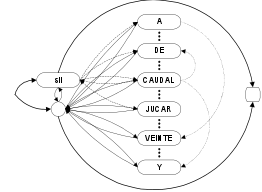
\includegraphics[scale=0.75]{fig03}}
	\caption[Ejemplo de gráfica flotante $\gamma$]{Ejemplo de gráfica flotante dos $\gamma$.} % El texto en corchetes será el texto que aparecerá en la lista de figuras. El texto en llaves será el que aparecerá debajo de la imagen.
	\label{fig:fig03}
\end{figure}

Para mejor calidad de impresión y electrónica se recomienda utilizar gráficos vectorizados. Por tanto guarde las imágenes directamente con formato ESP desde \emph{matlab} (para las gráficas utilice el formato de matlab adjunto), o bien, si se trata de una fotografía o imagen distinta utilice un convertidor de formatos sin perdidas de información a EPS. El nombre de cada imagen debe ir en minúscula, sin espacio entre palabras y sin caracteres acentuados para evitar errores posteriores.\\
A continuación se muestra la referencia a una figura compuesta por multiples sub-figuras como en la gráfica~\vref{fig:fig08}. Reference one of the subfigures as Figure~\vref{fig:fig05}.

\begin{figure}[tb]
	\centering
	\subfloat[Señal uno.]{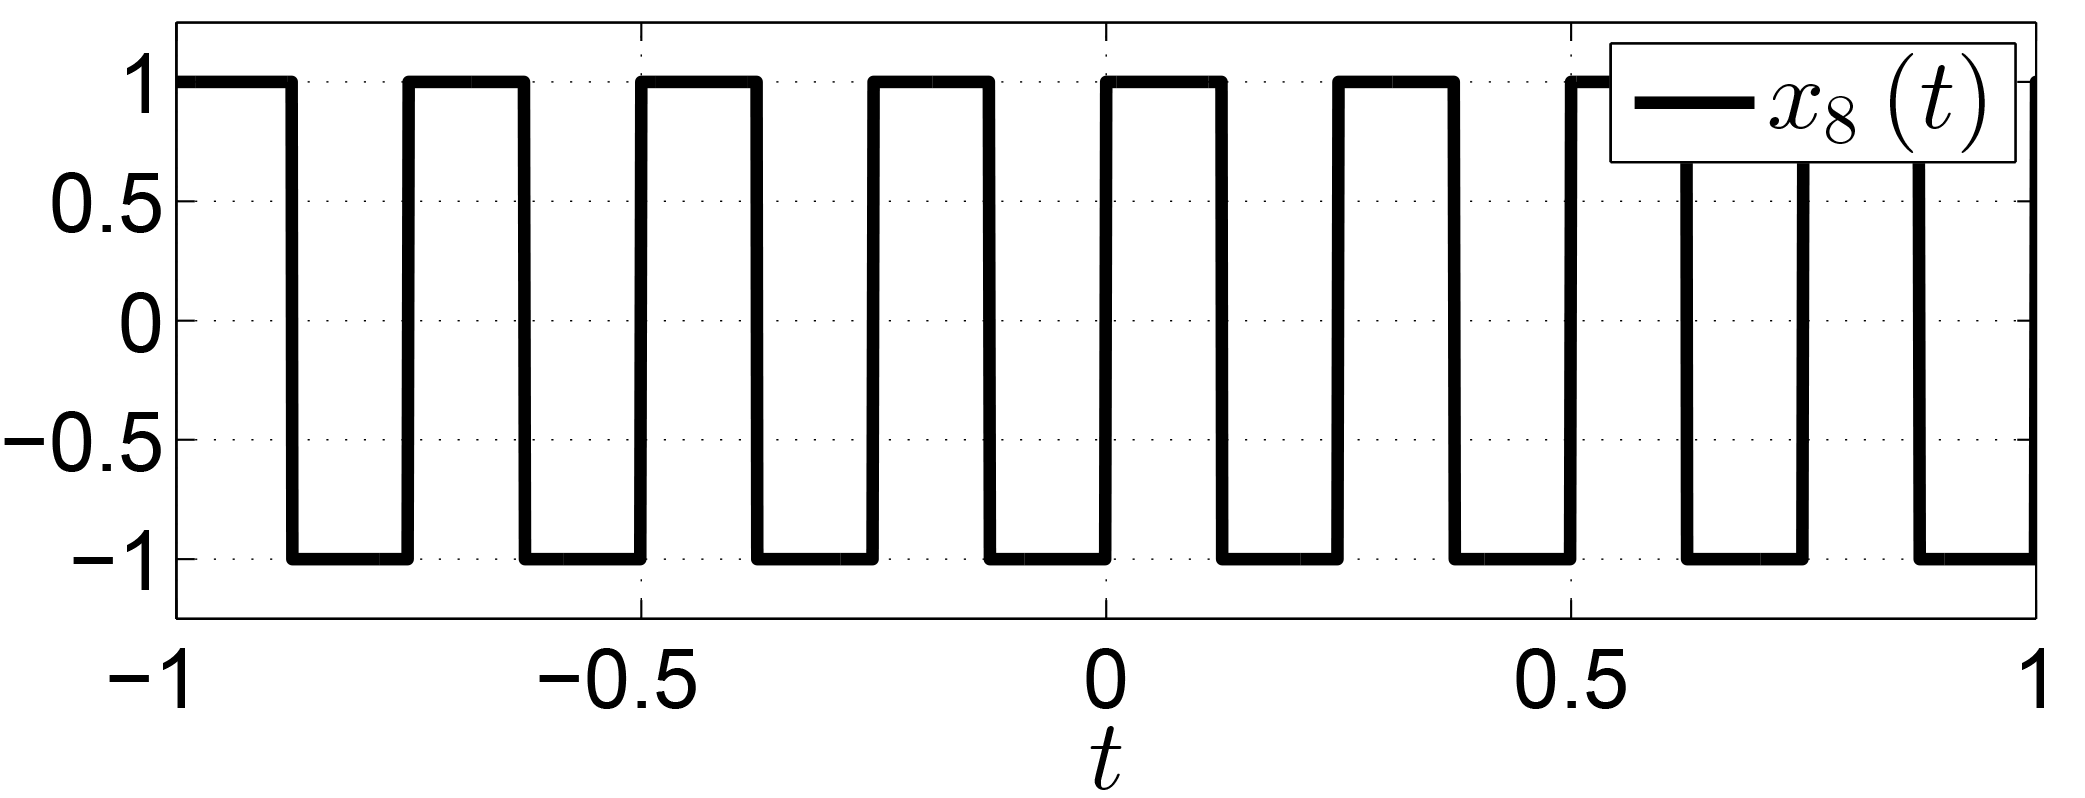
\includegraphics[width=.45\columnwidth]{fig04}} \quad
	\subfloat[Señal dos]{
\includegraphics[width=.45\columnwidth]{fig05}\label{fig:fig05}}\\
	\subfloat[Señal tres.]{
\includegraphics[width=.45\columnwidth]{fig06}} \quad
	\subfloat[Señal cuatro.]{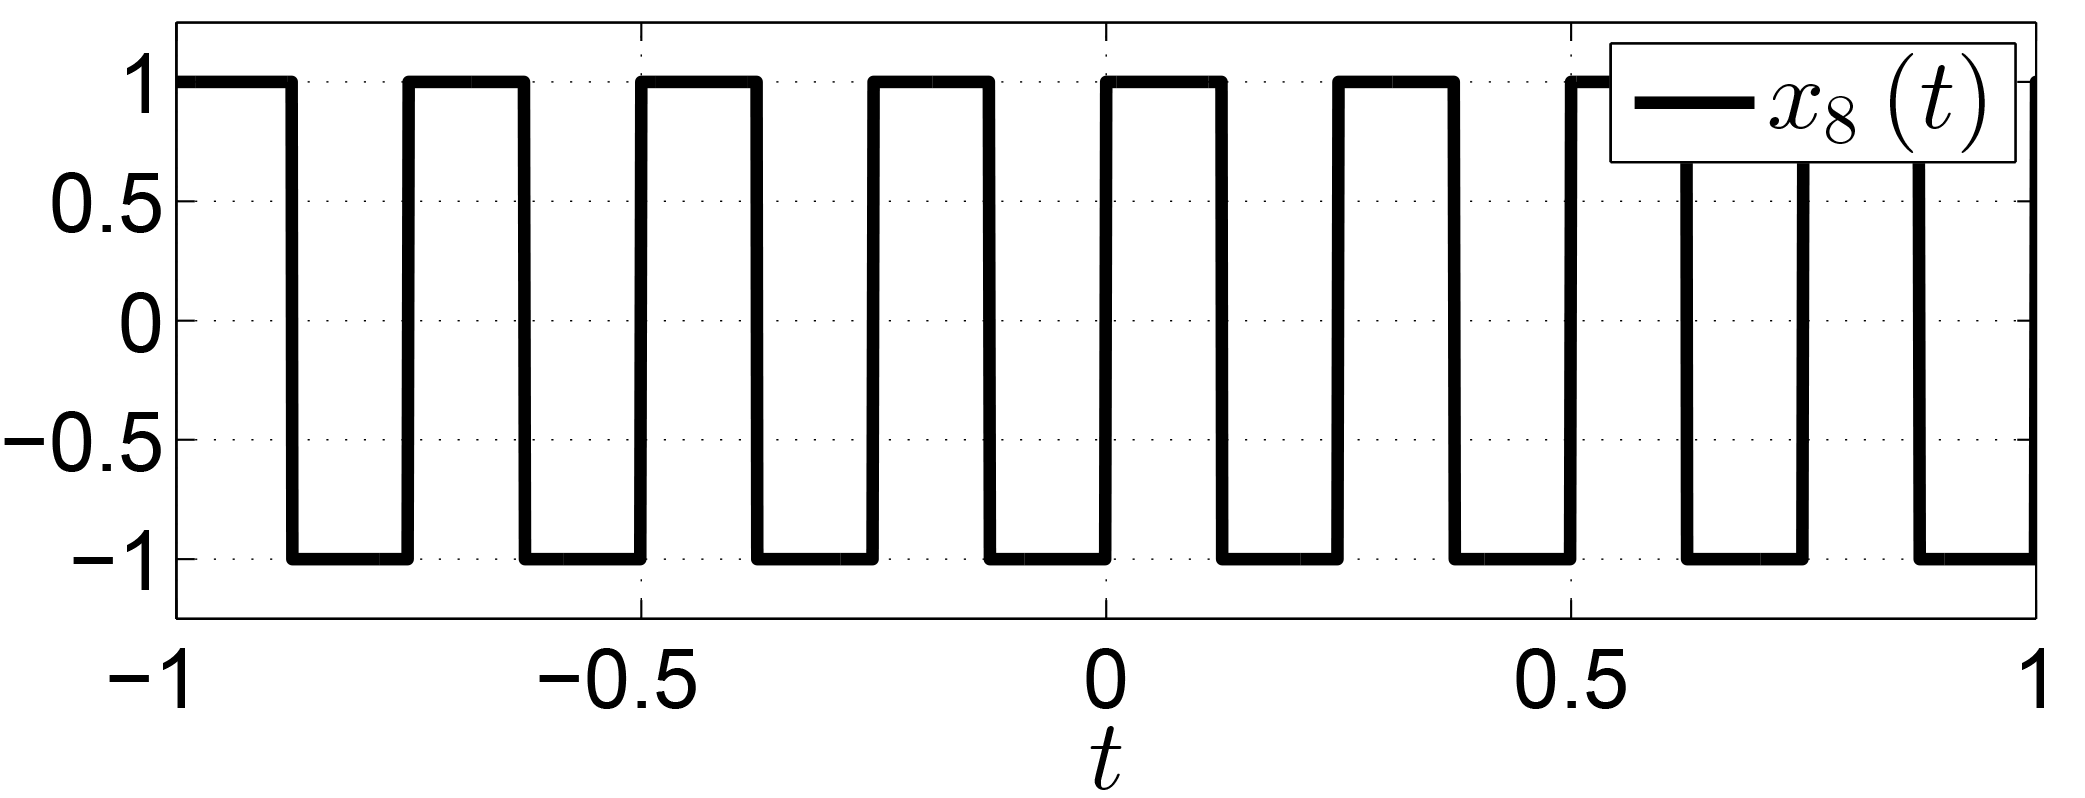
\includegraphics[width=.45\columnwidth]{fig07}}
	\caption[Composición de gráficas.]{Composición de gráficas.} % El texto en corchetes será el texto que aparecerá en la lista de figuras. El texto en llaves será el que aparecerá debajo de la imagen.
	\label{fig:fig08}
\end{figure}


\subsection{Matemática y formulas}

La matemática dentro del texto es recomendable escribirla de la forma siguiente: $\cos\pi=-1$ and $\alpha$. Las ecuaciones no muy grandes, definiciones de variables, alfabeto griego, pueden insertarse directamente en la línea del párrafo. Otro ejemplo sería $\textrm{{\textbf{h}}}_i^n = w_{i - 1} ,w_{i - 2}, \ldots,w_{i - n + 1}$ asociada un símbolo $w_i$.\\
Cuando se desea trabajar con ecuaciones más complejas para desarrollo, se recomienda utilizar el formato que se describe a continuación en un párrafo aparte:

\begin{equation}
\hat {P}_I (w_i \vert \textrm{{\textbf{h}}}_i^k ) = \sum\limits_{j=0}^{k-1} 
{\lambda _j \hat {P}(w_i \vert \textrm{{\textbf{h}}}_i^j ).} 
\label{eq:eq1}
\end{equation}

Según las normas internacionales, todas las formulas con referencia en el texto deben ser numeradas. Si se tiene que escribir una formula o un desarrollo matemático y esta a su vez no es de relevancia, no se numera. Se recomienda utilizar el siguiente comando para que solo se enumeren las formulas a las que usted haga referencia.\\
Para hacer referencia a esta ecuación desde el texto se menciona, por ejemplo, en la ecuación (\ref{eq:eq1}).\\
Si la formula no es relevante y es parte de un desarrollo, se escribe como de describe a continuación, colocando el símbolo asterisco a la función \textit{equation}.
\begin{equation*}
P\left(A=2\middle|\frac{A^2}{B}>4\right)=\left.\frac{A^3}{3}\right|_0^1 \frac{n!}{r!(n-r)!} \quad \text{si $n$ es par}.
\end{equation*}

Si al final de una formula empieza el texto nuevamente, se escribe un punto. Si después de la formula sigue otra fórmula se separan por punto y coma, tal cual como se observa en las ecuaciones~\ref{eq:eq2} y~\ref{eq:eq3}. La última formula de la lista (formula~\ref{eq:eq4}) lleva un punto.

\begin{equation}
\cos^3 \theta =\frac{1}{4}\cos\theta+\frac{3}{4}\cos 3\theta;
\label{eq:eq2}
\end{equation}

\begin{equation}
\cos^3 \theta =\frac{1}{4}\cos\theta+\frac{3}{4}\cos 3\theta;
\label{eq:eq3}
\end{equation}

\begin{equation}
\cos^3 \theta =\frac{3}{4}\cos\theta+\frac{1}{4}\sin 3\theta.
\label{eq:eq4}
\end{equation}

La explicación de las variables que intervienen en una formula se hace como se muestra a continuación. Después de cada descripción de variable se coloca un punto y coma, en la variable final se coloca un punto. Un ejemplo se puede observar en las formula siguiente~\ref{eq:eq5},
\begin{equation}
z = r\cdot\exp\left({j\varphi}\right),
\label{eq:eq5}
\end{equation}

\begin{table}[ht]
	\begin{tabular*} {1.0\linewidth}{lrcl}
		donde,	& $\varphi$	& "---	& fase del numero complejo;\\
		& $j$		& "---	& variable comleja.
	\end{tabular*}
\end{table}

A continuación veremos una ecuación de más de un renglón. Es necesario prestar atención a que las primeras dos formulas~\ref{eq:eq6} y~\ref{eq:eq7} están numeradas, mientras que la ecuación larga~\ref{eq:eq8}, el primer renglón no lo esta y se toma la formula en conjunto. También se puede apreciar que debajo de una gran formula se puede escribir una descripción.

\begin{eqnarray} 
S_{\text{out}}(x_2, y_2) = \iint dx_0 dy_0 A_0 g(x_0, y_0) \cdot h(x_2-x_0, y_2 -y_0) =     \label{eq:eq6} \\
= A_0 \underbrace{\iint dx_0 dy_0 \; g(x_0, y_0) 
	\cdot h(x_2-x_0, y_2 -y_0)}_{\text{por definición, esto es la convolución }} = A_0 g     \otimes h 
\label{eq:eq7}
\end{eqnarray}


\begin{eqnarray}
J_\lambda(x_2, y_2, s_2) =
\iint K_\lambda(x_2, y_2) \cdot \Bigl| m_\lambda
\left(
\frac{x_2-x_0}{\lambda \cdot s_2} , \frac{y_2-y_0}{\lambda \cdot s_2}\right)\Bigr|^2 \,dx_0\,dy_0 = \nonumber \\ %Sin numeración
= K_\lambda(x_2, y_2) \otimes \Bigl| m_\lambda \left( \frac{x_2}{\lambda \cdot s_2} , \frac{y_2}{\lambda \cdot s_2} \right) \Bigr|^2.
\label{eq:eq8}
\end{eqnarray}

Otra forma de escribir una ecuación por partes es mediante el comando \emph{matrix} (ecuación~\ref{eq:eq9}).

\begin{equation}
\begin{matrix}
\hat{\Phi}[k,l] & = & \left\{
\begin{matrix}
0 & \mbox{if } k,l = 0 \\
S_x[k,l]\cdot H_x[k,l] + S_y[k,l]\cdot H_y[k,l] & \mbox{otherwise }
\end{matrix} 
\right.
\end{matrix}
\label{eq:eq9}
\end{equation}

Otra forma de escribir muchas ecuaciones es mediante el comando \emph{align}, este comando es muy útil para el desarrollo de ejercicios, demostraciones, etc. que requieran además textos intermedios de explicaciones. La ecuación por partes se realiza mediante el comando \emph{cases} (ecuación~\ref{eq:eq10}).
\begin{align}
\begin{cases}
\dot{x}=-R\omega\sin\omega t\\
\dot{y}=\hphantom{-}R\omega\cos\omega t
\end{cases}
\label{eq:eq10}\\
\intertext{por consiguiente,}
a_{\tau}=0
\label{eq:eq11}
\end{align}

Un ejemplo de ecuación por partes con condicionales se expresa mediante:
\begin{numcases}{|x|=}
x, & para $x \geq 0$;\\
-x, & para $x < 0$.
\end{numcases}

A continuación un ejemplo de teorema~\ref{th:th01} expresado de acuerdo al formato
\begin{thm}[Pitágoras]
	En todo triángulo rectángulo el cuadrado de la hipotenusa es igual a la suma de los cuadrados de los catetos.
	\label{th:th01}
\end{thm}

Las demostraciones pueden ser escritas mediante los comandos del siguiente ejemplo:

\begin{proof} 
	Se tiene que $\log(1)^2 = 2\log(1)$. Pero tambien se conoce que $\log(-1)^2=\log(1)=0$. Entonces $2\log(-1)=0$, por lo cual se prueba. 
\end{proof}

Otros ejemplos de matemáticas se muestran a continuación:
\begin{equation*}
\frac{1}{1+
	\frac{1}{1+
		\frac{1}{1+
			\frac{1}{2}}}}
\end{equation*}

Para mayor tamaño se utiliza el comando \emph{displaystyle}.

\begin{equation*}
\frac{1}{\displaystyle 1+
	\frac{1}{\displaystyle 1+
		\frac{1}{\displaystyle 1+
			\frac{\displaystyle 1}
			{\displaystyle 2}}}}
\end{equation*}

El index de algunas variables se puede escribir como se muestra a continuación:

\[A_{\text{indice inferior}}\quad
B^{\text{indice superior}}\quad
C_n^k\]

Ejemplo de derivadas:

\[ f'\quad f''\quad f''' \quad f^n \]
\[\dot{x}\quad \ddot{x}\quad \ddot{x}\]
\[\frac{d f}{d x}\quad
\frac{d^n f}{d x^n}\quad
\frac{\partial^2 f}{\partial x\partial y}\]

Ejemplo de integrales y sumas:
\[
\int_0^{\infty}\quad
\int\limits_0^{\infty}\quad
\sum_{i=1}^n\quad
\sum\nolimits_{i=1}^n\quad
\]

\section{Tablas}

Un ejemplo de una tabla de estilo sencillo puede verse a continuación en la tabla~\ref{tab:tab1}.

\begin{table}[htbp]
	\caption{Nombre de la tabla sencilla.}
	\begin{center}
		\begin{tabular}{l|c|c|c|c}
			\toprule
			Errores de     & SER    & WER  & WAER & Reducción \\
			reconocimiento & {\%}   & {\%} & {\%} & {\%}WER   \\
			\hline
			Referencia& 38.30& 7.54& 8.53&    -- \\
			HMM-PASS  & 30.55& 5.36& 6.67& 28.91 \\
			T-PASS    & 25.50& 4.76& 5.70& 36.87 \\
			\bottomrule
		\end{tabular}
	\end{center}
	\label{tab:tab1}
\end{table}
Todas las tablas deben tener enlaces de referencia dentro del texto. A continuación se tiene una tabla (ver tab.~\ref{tab:tab2}) con filas y columnas complejas.

\begin{table}[hbt]
	\caption{Nombre de la tabla compleja.}
	\begin{center}
		\begin{tabular}{llr}
			\toprule
			\multicolumn{2}{c}{Name} \\
			\cmidrule(r){1-2}
			First name & Last Name & Grade \\
			\midrule
			John & Doe & $7.5$ \\
			Richard & Miles & $2$ \\
			\bottomrule
		\end{tabular}
	\end{center}
	\label{tab:tab2}
\end{table}

%\end{comment}
\section{Códigos}

A continuación un ejemplo de inserción de código sencillo en el código~\ref{lst:ffjk}. Hay que tener en cuenta el tipo de codificación a utilizar, en el ejemplo se muestra un tipo de código implementado en \textit{VHDL}.
\begin{lstlisting}[language=VHDL, caption={Proceso que implementa un biestable J-K},label={lst:ffjk}]
P_JK1: Process (Clk)
begin
if Clk'event and Clk='1' then
if J='1' and K='1' then
Q <= not Q;
elsif J='1' and K='0' then
Q <= '1';
elsif J='0' and K='1' then
Q <= '0';
else
Q <= Q;
end if;
end if;
end process;
\end{lstlisting}

\subsection{Códigos de Matlab}
Existen tres formas de implementar códigos de \textit{Matlab}. Pero para ello es necesario haber llamado el paquete de códigos de \textit{Matlab} \verb|\mcode{}|.\\
1) El bloque del código~\ref{lst:codmatlab} se implementa utilizando el paquete de entorno \verb|lstlisting|.
\begin{lstlisting}[language=matlab,caption={Código Matlab que hace algo},label={lst:codmatlab}]
for i = 1:3
if i >= 5 && a ~= b       % literate programming replacement
disp('cool');           % comment with some §\mcommentfont\LaTeX in it: $\mcommentfont\pi x^2$§
end
[:,ind] = max(vec);
x_last = x(1,end) - 1;
v(end);
really really long really really long really really long really really long really really long line % blaaaaaaaa
ylabel('Voltage (µV)');
end
\end{lstlisting}
2) Se puede utilizar código dentro del texto y párrafos tal cual como se lee a continuación  \mcode{for i=1:3, disp('cool'); end;} usando el comando \verb|\mcode{}|.\footnote{También es posible para pies de página: \mcodefn{for i=1:3, disp('cool'); end;}}\\
3) Es posible insertar código directamente desde un archivo externo de extensión \textit{.m} guardado en alguna parte del disco duro. El código completo implementado en \textsc{Matlab}, usando la siguiente linea de comando \verb|\lstinputlisting{/ALGUNA/CARPETA/Archivo.m}|. Si solo se desea incluir una parte (solo algunas lienas) de ese archivo de \textsc{Matlab} (no incluyendo encabezados, etc.) se puede utilizar el siguiente comando \verb|\lstinputlisting[firstline=6, lastline=15]{/SOME/PATH/FILENAME.M}|.
%\lstinputlisting{/path_to_mfile/my_mfile.m}
\section{Diagrama bloques y circuitos}

Para dibujar diagramas de bloques en \LaTeX \, es recomendable utilizar el paquete tikzpicture. Este permite dibujar diagramas sin mayor dificultad. Un ajemplo de bloque sencillo se puede observar en la figura~\ref{fig:diag01}. Se recomienda leer en los archivos adjuntos acerca del paquete correspondiente y su utilización. A continuación tambien se muestran ejemplos de diagrama de bloques en las figuras~\ref{fig:diag03}~y~\ref{fig:diag03}. 

\begin{figure}[tbhp]
	\centering
	\begin{minipage}{1.0\textwidth}
		\centering
		\begin{tikzpicture}[scale=1]
		\sbEntree{start}
		\sbBloc{block}{Bloque}{start} %Definición del bloque
		\sbRelier[Entrada \Spacing \Spacing]{start}{block}
		\sbSortie{end}{block}
		\sbRelier[\Spacing \Spacing Salida]{block}{end}
		\end{tikzpicture}
		\caption[Ejemplo de bloque sencillo]{Ejemplo de bloque sencillo.}
		\label{fig:diag01}
	\end{minipage}%
\end{figure}


\begin{figure}[tbhp]
	\centering
	\begin{minipage}{1.0\textwidth}
		\centering
		\begin{tikzpicture}[scale=1]
		\sbEntree{E}
		\sbBlocL[5]{H1}{$H_1$}{E}
		\sbBlocL{H2}{$H_2$}{H1}
		\sbDecaleNoeudy[4]{H2}{H3}
		\sbBloc[3]{H3}{$H_3$}{H3}
		\sbRelierxy[aa]{H2}{H3}
		
		\sbDecaleNoeudy[10]{H2}{H4}
		\sbBloc[3]{H4}{$H_4$}{H4}
		\sbRelier[bb]{H3}{H4}
		
		\sbDecaleNoeudy[4]{H4}{H5}
		\sbBloc[3]{H5}{$H_5$}{H5}
		\sbRelieryx{H4}{H5} 
		
		\sbBlocL{H6}{$H_6$}{H5}
		
		\end{tikzpicture}
		\caption[Ejemplo de bloque sencillo]{Ejemplo de bloque sencillo.}
		\label{fig:diag02}
	\end{minipage}%
\end{figure}

\begin{figure}[tbhp]
	\centering
	\begin{minipage}{1.0\textwidth}
		\centering
		\begin{tikzpicture}[scale=1]
		\sbEntree{E}
		\sbComp{a}{E}
		\sbBloc{b}{$H_1$}{a}
		\sbRelier[$E_1$]{E}{a}
		\sbBlocL{c}{$H_2$}{b}
		\sbRelier[$\epsilon$]{a}{b}
		\sbComph{d}{c}
		\sbRelier[u]{c}{d}
		\sbBlocL{e}{$H_3$}{d}
		\sbBlocL{f}{$H_4$}{e}
		\sbSortie[5]{S1}{f}
		\sbRelier{f}{S1}
		\sbNomLien[0.8]{S1}{$S_1$}
		\sbDecaleNoeudy[-4]{f}{u}
		\sbDecaleNoeudy{e}{v}
		\sbBlocr{r1}{$R_1$}{u}
		\sbBlocr{r2}{$R_2$}{v}
		\sbBlocrL{r3}{$R_3$}{r2}
		\sbRelieryx{f-S1}{r1}
		\sbRelierxy[n1]{r1}{d}
		\sbRelieryx{e-f}{r2}
		\sbRelierxy[n2]{r3}{a}
		\end{tikzpicture}
		\caption[Diagrama de bloques]{Diagrama de bloques.}
		\label{fig:diag03}
	\end{minipage}%
\end{figure}


% http://tug.ctan.org/tex-archive/graphics/pgf/contrib/schemabloc/
% http://sciences-indus-cpge.papanicola.info/Schema-blocs-avec-PGF-TIKZ-sous
% http://bay.uchicago.edu/CTAN/graphics/pgf/contrib/schemabloc/

\section{Recomendaciones generales}

Defina adecuadamente cada una de las abreviaturas a utilizar, los acrónimos y símbolos que utilizará la primera vez que aparece en el texto (con excepción del resumen), por ejemplo, relación señal ruido (SNR). Luego utilice este acrónimo en lugar de escribir completamente el término.

Aclaré mediante notación cuando utilice operadores matemáticos especiales y poco frecuentes. No olvide la importancia de definir cada variable que aparece en las ecuaciones la primera vez.

\subsection{Formato de envío electrónico y físico}

El trabajo debe ser enviado antes de la fecha indicada por medio electrónico. El PDF resultante debe ser impreso y entregado por escrito el día designado para ello.\\
Para nombrar la carpeta, el archivo \LaTeX del proyecto y el asunto del correo electrónico es necesario utilizar el siguiente formato: El "Nombredelproyecto" se llamará de acuerdo a la siguiente construcción \textbf{CODtrabajo-CODGrupoEstudiante-CODtrabajo}.\\
El estudiante esta en deber de conocer estos datos antes de enviar su trabajo. La carpeta Nombredelproyecto debe contener:
\begin{itemize}[noitemsep] % noitemsep elimina los espacios en blanco entre los elementos dando así aspecto compacto.
	\item Archivo Nombredelproyecto.tex;
	\item Archivo structure.tex; %Archivo de estructuras
	\item Archivo biblio.bib; %Archivo de biblioteca
	\item Carpeta llamada Figures, con todas las imágenes incluidas en el trabajo;
	\item Carpeta llamada Codes, con todos los códigos utilizados para realizar el trabajo, inclusive los de generación de gráficas.
\end{itemize}

Luego se comprimirá en un archivo ZIP la carpeta raíz (principal). El archivo comprimido enviará adjunto al correo electrónico \url{marco.teran@usa.edu.co}. El asunto del correo electrónico será Nombredelproyecto. El docente debe compilar el archivo .tex en su computador y se debe generar el PDF automaticamente sin errores.
Se recomienda compilar (build) mediante pdflatex.


\section{Conclusiones}

Es obligatorio que todos los trabajos tengan conclusiones.
Esta debe contener una revisión de todos los temas claves del trabajo.
Esta a su vez debe presentar el análisis de los resultados que se obtuvieron. Esta sección NO es un resumen.\\
Recuerde que pésimas conclusiones le quitarán importancia a todo el esfuerzo y trabajo realizado durante el laboratorio.


\section{Citas bibliográficas}

El estudiante debe establecer claramente la autoría de su trabajo. 
Los trabajos deben presentar referencias, deben estar claramente documentados, con sus respectivas citas independientemente de fuente bibliográfica utilizada. Todas las fuentes bibliográficas deberán ser indexadas (ISBN, DOI, etc.).
Incluso en el caso de utilizar una fuente con licencia de dominio público o Copyleft, (Ver: \url{http://creativecommons.org/}), el estudiante debe proporcionar la atribución de ese trabajo con el fin de mantener las políticas de autoría y modelos de contratos de licenciamiento. Toda la información que usted propone en este documento debe tener fuentes bibliográficas. Estas deben estar enlazadas a los apartados del texto donde se les hace referencias. El enlace se escribe tal cual como se muestra a continuación \cite{Tufte2006}.
. Es de suma importancia dejar en claro las pautas y el formato necesario para escribir bibliografía de forma correcta. En caso de que el texto o frase del documento requiera nota al pie, se puede realizar tal cual como se muestra aquí \footnote{Un ejemplo de nota al pie}. Es posible establecer una cita de la siguiente forma \cite{Tufte2006,Tufte1990}.\\

%----------------------------------------------------------------------------------------
%	Bibliografía
%----------------------------------------------------------------------------------------
\nocite{*}
\bibliography{biblio}
\bibliographystyle{unsrt}


\end{document}